% !TEX encoding = UTF-8 Unicode

\documentclass[a4paper]{article}

\usepackage{color}
\usepackage{url}
\usepackage[utf8]{inputenc}
\usepackage{graphicx}
\usepackage[english,serbian]{babel}
\usepackage[unicode]{hyperref}
\usepackage{amsmath}
\usepackage{amsthm}
\usepackage{amssymb}
\hypersetup{colorlinks,citecolor=green,filecolor=green,linkcolor=blue,urlcolor=blue}
\usepackage[title]{appendix}
\usepackage{float}
\usepackage[graphicx]{realboxes}
\usepackage[font=small,labelfont=bf]{caption}
\usepackage{chngcntr}
\counterwithin{figure}{section}
\usepackage{listings}
\usepackage{textcomp}
\usepackage{xcolor}
\lstset {
    language=C++,
    frame=single,
    framesep=10pt,
    tabsize=4,
    showstringspaces=false,
    upquote=true,
    commentstyle=\color{commentgreen},
    keywordstyle=\color{orange},
    stringstyle=\color{red},
    basicstyle=\small\ttfamily,
    emph={int,char,double,float,unsigned,void,bool},
    emphstyle={\color{blue}},
    escapechar=\&,
    % keyword highlighting
    classoffset=1, % starting new class
    morekeywords={>,<,.,;,,,-,!,=,~},
    keywordstyle=\color{weborange},
    classoffset=0,
}


\begin{document}

\title{Binarni dijagrami odlu\v{c}ivanja\\ \small{Seminarski rad u okviru kursa\\Automatsko rezonovanje\\ Matematički fakultet}}

\author{\href{mailto:mi14031@matf.bg.ac.rs}{Milana Kova\v{c}evi\'c}\\\href{mailto:mi14042@matf.bg.ac.rs}{Ivan Ristovi\'c}}
\date{jul 2018.}

\maketitle

\emph{Binarni dijagrami odlu\v{c}ivanja} (u daljem tekstu \emph{BDD}) i njihova pobolj\v{s}anja su strukture podataka za reprezentaciju bulovskih funkcija. Iako u osnovi sli\v{c}ni binarnim drvetima, re\v{s}avaju problem velikog broja \v{c}vorova u drvetu uklanjaju\'c{}i redundantne grane (za bulovsku funkciju sa $n$ argumenata, broj mogu\'c{}ih puteva u binarnom drvetu od korena do lista je $2^{n}$, dok je broj \v{c}vorova znatno ve\'c{}i). U ovom radu \'c{}emo detaljnije opisati ideju na kojoj su zasnovani BDD, na\v{c}ine za njihovu konstrukciju, kao i razne varijante BDD - \emph{ROBDD}, \emph{FBDD} i \emph{ZDD}. Ovaj rad \'c{}e pratiti implementacija ROBDD u jeziku \emph{C++}, uz prate\'c{}e delove koda na nekim mestima.


\tableofcontents

\newpage

\section{Bulovske funkcije}
\label{sec:BulovskeFunkcije}

\emph{Bulovske funkcije} su funkcije koje primaju argumente koji su bulovske vrednosti i vra\'c{}aju bulovsku vrednost. Bulovske vrednosti mogu biti \emph{true} ili \emph{false}. U nastavku \'c{}emo sa $1$ ozna\v{c}avati \emph{true}, a sa $0$ \emph{false}, \v{s}to je uobi\v{c}ajena konvencija.

Za bulovsku funkciju sa $n$ bulovskih argumenata, postoji $2^{n}$ mogu\'c{}ih ulaza. Po\v{s}to je povratna vrednost takodje bulovskog tipa, zaklju\v{c}ujemo da postoji $2^{2^{n}}$ razli\v{c}itih bulovskih funkcija sa $n$ argumenata, \v{s}to se vidi iz jednakosti

\[ \underbrace{2*2*2* \dotsb *2}_{\text{$2^{n}$}} = 2^{2^{n}} \]

Funkcije koje primaju neozna\v{c}eni broj u opsegu $[0,2^{n}-1]$ se mogu zameniti sa $n$ bulovskih funkcija sa $n$ argumenata. Kao primer, neka je data funkcija $F$ koja prima i vra\'c{}a neozna\v{c}eni ceo broj. Zamenjujemo funkciju $F$ bulovskim funkcijama $f_i$, $i = 0, 1, \dots , n-1$. Argumenti funkcije $f_{i}$ su $n$ binarnih cifara broja, dok je povratna vrednost $f_{i}$ vrednost $i$-te binarne cifre rezultata funkcije $F$. Drugim re\v{c}ima, svaka od funkcija $f_{i}$ ra\v{c}una jednu cifru rezultata. Kao konkretan primer, s obzirom da su neozna\v{c}eni brojevi u ra\v{c}unarima zauzimaju obi\v{c}no $32$ bita, funkciju

\begin{lstlisting}[language=C++]
    unsigned F(unsigned n);
\end{lstlisting}

\noindent mo\v{z}emo zameniti sa $32$ bulovske funkcije

\begin{lstlisting}[language=C, emph={bool}]
    bool f0(bool n0, bool n1, bool n2, ... , bool n31);
    bool f1(bool n0, bool n1, bool n2, ... , bool n31);
    ...
    bool f31(bool n0, bool n1, bool n2, ... , bool n31);
\end{lstlisting}

Naravno, moramo se uveriti da su cifre rezultata zaista jednake izlazima bulovskih funkcija. Jedan na\v{c}in za verifikaciju rezultata je primena obe tehnike nad svim mogu\'c{}im ulazima i poredjenje dobijenih rezultata. Medjutim, \v{c}ak i za ovako jednostavne funkcije re\v{c} je o oko 4 milijarde ($2^{32}$) mogu\'c{}ih ulaza. Drugi na\v{c}in je da se ove funkcije prika\v{z}u putem nekih struktura podataka, i da se funkcije porede tako \v{s}to se porede njihove reprezentacije preko tih struktura. Drugim re\v{c}ima, posmatramo funkcije kao podatke. U poglavljima koji slede \'c{}e biti vi\v{s}e re\v{c}i o strukturama podataka koje se koriste za predstavljanje bulovskih funkcija. Takodje, u narednim poglavljima pod terminom \emph{funkcija} \'c{}emo podrazumevati bulovske funkcije, ukoliko to nije druga\v{c}ije nazna\v{c}eno.

\section{Binarna drveta odlu\v{c}ivanja}
\label{sec:BinarnaDrvetaOdlucivanja}

Binarna drveta odlu\v{c}ivanja su u osnovi jako sli\v{c}na binarnim drvetima. Na ovom nivou radimo sa bulovskim funkcijama. Neka je dato $n$ promenljivih $x_{1}, x_{2}, \dots , x_{n}$ koje predstavljaju ulaze u bulovsku funkciju $f$. U korenom \v{c}voru testiramo jednu promenljivu (bez umanjenja op\v{s}tosti, krenu\'c{}emo redom, te neka je to $x_{1}$). U zavisnosti od vrednosti te promenljive formiraju se dva pod-drveta - jedno u kome je $x_{1} = 0$ (\emph{nisko} pod-drvo), a drugo u kome je $x_{1} = 1$ (\emph{visoko} pod-drvo). U svakom pod-drvetu se rekurzivno testiraju ostale promenljive na isti na\v{c}in. Do listova se dolazi kada vi\v{s}e nema preostalih ulaznih promenljivih. Posmatraju\'c{}i jedan put od korena do lista, dobijamo valuaciju za skup $\{x_{1}, \dots , x_{n}\}$.

Uzmimo za primer funkciju:

\begin{lstlisting}[language=C++]
    bool f_and(bool x1, bool x2) { return x1 && x2; }
\end{lstlisting}

\noindent Matematički zapis ove funkcije bi bio $x_{1} \wedge x_{2}$. Binarno drvo odlu\v{c}ivanja za ovu funkciju je dat na slici \ref{diag:BDAnd}. Polaze\'c{}i od promenljive $x_{1}$, formiramo dve grane na osnovu toga da li je $x_{1} = 0$ ili $x_{1} = 1$. Od sada pa u budu\'c{}e \'c{}emo grane u kojima je vrednost $0$ crtati isprekidanom linijom, a grane u kojima je vrednost $1$ punom linijom, zarad preglednosti.

\begin{figure}[H]
    \centering
    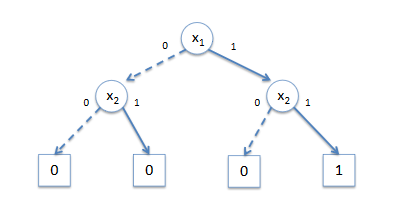
\includegraphics[scale=0.8]{slike/BD_And.PNG}
    \caption{Binarno drvo odlu\v{c}ivanja za funkciju $\wedge$}
    \label{diag:BDAnd}
\end{figure}

\noindent Sli\v{c}no se mogu definisati i ostale korisne funkcije, na primer \texttt{f\_or} ($\vee$) i \texttt{f\_xor} ($\oplus$), sa dijagramima na slici \ref{fig:BDOrXor}:

\begin{lstlisting}[language=C++,escapechar=@]
    bool f_or(bool x1, bool x2) { return x1 || x2; }

    bool f_xor(bool x1, bool x2) {
        return (x1 && !x2) || (!x1 && x2); @\footnote{Ne mo\v{z}emo koristiti operator \^{} jer on operi\v{s}e nad promenljivima tipa \emph{int}, a ne \emph{bool}.}@
    }
\end{lstlisting}

\begin{figure}[H]
    % NE DIRAJ OVE BROJEVE
    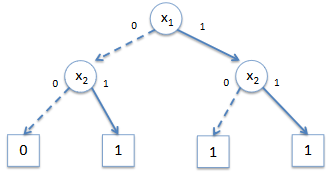
\includegraphics[scale=0.68]{slike/BD_Or.PNG}
    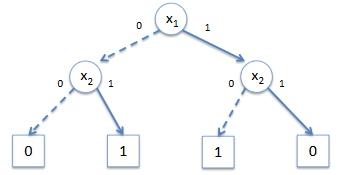
\includegraphics[scale=0.68]{slike/BD_Xor.PNG}
    \caption{Binarna drveta odlu\v{c}ivanja za funkcije $\vee$ i $\oplus$, redom}
    \label{fig:BDOrXor}
\end{figure}

Binarna drveta odlu\v{c}ivanja imaju neke veoma lo\v{s}e osobine. Najve\'c{}i problem je njihova veli\v{c}ina. Binarno drvo za $n$ ulaznih promenljivih \'c{}e imati $2^{n-1}$ unutra\v{s}njih \v{c}vorova i $2^{n}$ listova.

Uprkos tome, postoje i neke dobre osobine, pre svega \emph{kanoni\v{c}nost}. Ukoliko testiramo promenljive uvek u istom redosledu (tada se binarno drvo odlu\v{c}ivanja naziva \emph{uredjeno}), onda je drvo jedinstveno za svaku bulovsku funkciju. Stoga se test ekvivalencije dve bulovske funkcije svodi na testiranje ekvivalentnosti njivohih binarnih drveta odlu\v{c}ivanja. Na\v{z}alost, zbog velikog broja \v{c}vorova u drvetima, problem je eksponencijalne slo\v{z}enosti u odnosu na broj ulaznih parametara.

Kako bi se re\v{s}io problem eksplozije broja \v{c}vorova u drvetu, formiraju se unapredjenja binarnih drveta odlu\v{c}ivanja - binarni dijagrami odlu\v{c}ivanja (\emph{BDD}). O njima \'c{}e biti vi\v{s}e re\v{c}i u poglavlju koje sledi.

\section{Binarni dijagrami odlu\v{c}ivanja}
\label{sec:BDD}

Binarni dijagrami odlu\v{c}ivanja (engl. \emph{Binary Decision Diagrams}, u daljem tekstu \emph{BDD}) su unapredjenje binarnih drveta odlu\v{c}ivanja. Prvo unapredjenje je uklanjanje redundantnih grana u drvetu. Na primer, posmatrajmo funkciju $\wedge$ definisanu u poglavlju \ref{sec:BinarnaDrvetaOdlucivanja}. U niskom pod-drvetu obe grane koje polaze od promenljive $x_{2}$ vode ka vrednosti $0$, stoga nije potrebno ispitivati vrednost promenljive $x_{2}$ \footnote{tzv. \emph{lenjo izra\v{c}unavanje}}. Ovakvom redukcijom se dobija drvo na slici \ref{diag:BDDAnd}.

\begin{figure}[H]
    \centering
    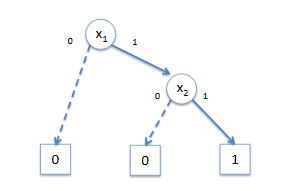
\includegraphics[scale=0.8]{slike/BDD_And.PNG}
    \caption{BDD za funkciju $\wedge$}
    \label{diag:BDDAnd}
\end{figure}

Drugo unapredjenje je dozvoljavanje deljenja identi\v{c}nih pod-drveta. Ponovo, kako bi \v{c}italac bolje razumeo \v{s}ta ovo zapravo zna\v{c}i, dajemo primer. Posmatrajmo funkciju koja ima povratnu vrednost $1$ ukoliko postoji neparan broj ulaznih promenljivih sa vredno\v{s}\'c{}u $1$, a $0$ ina\v{c}e. \v{S}tavi\v{s}e, pretpostavimo da imamo \v{c}etiri ulazne promenljive $x_{1}$, $x_{2}$, $x_{3}$ i $x_{4}$. Binarno drvo odlu\v{c}ivanja za ovakvu funkciju bi imalo 15 ($2^4 - 1$) unutra\v{s}njih \v{c}vorova i 16 ($2^4$) listova. Medjutim, BDD za ovu funkciju ima samo 7 unutra\v{s}njih \v{c}vorova i samo dva lista (slika \ref{diag:BDDParity}).

\begin{figure}[H]
    \centering
    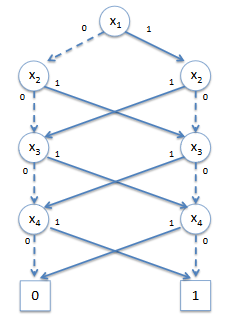
\includegraphics[scale=0.8]{slike/BDD_Parity.PNG}
    \caption{BDD za funkciju parnosti \v{c}etiri argumenta}
    \label{diag:BDDParity}
\end{figure}

U najgorem slu\v{c}aju, BDD \'c{}e biti eksponencijalno veliki u odnosu na ulaz, mada u praksi je to retko slu\v{c}aj. Takodje, konstantne funkcije se mogu predstaviti samo jednim \v{c}vorom, bez obzira na broj ulaznih promenljivih.


\addcontentsline{toc}{section}{Literatura}
\bibliographystyle{plain}
\bibliography{literatura}

\newpage

%\begin{appendices}
%\input{delovi/???}
%\end{appendices}

\end{document}
